\documentclass[bachelor, och, coursework]{SCWorks}
% параметр - тип обучения - одно из значений:
%    spec     - специальность
%    bachelor - бакалавриат (по умолчанию)
%    master   - магистратура
% параметр - форма обучения - одно из значений:
%    och   - очное (по умолчанию)
%    zaoch - заочное
% параметр - тип работы - одно из значений:
%    referat    - реферат
%    coursework - курсовая работа (по умолчанию)
%    diploma    - дипломная работа
%    pract      - отчет по практике
% параметр - включение шрифта
%    times    - включение шрифта Times New Roman (если установлен)
%               по умолчанию выключен
\usepackage{subfigure}
\usepackage{tikz,pgfplots}
\pgfplotsset{compat=1.5}
\usepackage{float}

%\usepackage{titlesec}
\setcounter{secnumdepth}{4}
%\titleformat{\paragraph}
%{\normalfont\normalsize}{\theparagraph}{1em}{}
%\titlespacing*{\paragraph}
%{35.5pt}{3.25ex plus 1ex minus .2ex}{1.5ex plus .2ex}

\titleformat{\paragraph}[block]
{\hspace{1.25cm}\normalfont}
{\theparagraph}{1ex}{}
\titlespacing{\paragraph}
{0cm}{2ex plus 1ex minus .2ex}{.4ex plus.2ex}

% --------------------------------------------------------------------------%


\usepackage[T2A]{fontenc}
\usepackage[utf8]{inputenc}
\usepackage{graphicx}
\graphicspath{ {./images/} }
\usepackage{tempora}

\usepackage[sort,compress]{cite}
\usepackage{amsmath}
\usepackage{amssymb}
\usepackage{amsthm}
\usepackage{fancyvrb}
\usepackage{listings}
\usepackage{listingsutf8}
\usepackage{longtable}
\usepackage{array}
\usepackage[english,russian]{babel}

%\usepackage[colorlinks=true]{hyperref}
\usepackage{url}

\usepackage{underscore}
\usepackage{setspace}
\usepackage{indentfirst} 
\usepackage{mathtools}
\usepackage{amsfonts}
\usepackage{enumitem}
\usepackage{tikz}
\usepackage{minted}
\newcommand{\eqdef}{\stackrel {\rm def}{=}}
\newcommand{\specialcell}[2][c]{%
\begin{tabular}[#1]{@{}c@{}}#2\end{tabular}}

\renewcommand\theFancyVerbLine{\small\arabic{FancyVerbLine}}

\newtheorem{lem}{Лемма}

\begin{document}

% Кафедра (в родительном падеже)
\chair{теоретических основ компьютерной безопасности и криптографии}

% Тема работы
\title{Исследование моделей рекомендательных систем}

% Курс
\course{3}

% Группа
\group{331}

% Факультет (в родительном падеже) (по умолчанию "факультета КНиИТ")
\department{факультета КНиИТ}

% Специальность/направление код - наименование
%\napravlenie{09.03.04 "--- Программная инженерия}
%\napravlenie{010500 "--- Математическое обеспечение и администрирование информационных систем}
%\napravlenie{230100 "--- Информатика и вычислительная техника}
%\napravlenie{231000 "--- Программная инженерия}
\napravlenie{100501 "--- Компьютерная безопасность}

% Для студентки. Для работы студента следующая команда не нужна.
% \studenttitle{Студентки}

% Фамилия, имя, отчество в родительном падеже
\author{Окунькова Сергея Викторовича}

% Заведующий кафедрой
\chtitle{доцент, к.ф.-м.н.} % степень, звание
\chname{М.~Б.~Абросимов}

%Научный руководитель (для реферата преподаватель проверяющий работу)
\satitle{Доцент} %должность, степень, звание
\saname{И. И. Слеповичев}

% Руководитель практики от организации (только для практики,
% для остальных типов работ не используется)
%\patitle{к.ф.-м.н.}
%\paname{М.~Б.~Абросимов}

% Семестр (только для практики, для остальных
% типов работ не используется)
%\term{8}

% Наименование практики (только для практики, для остальных
% типов работ не используется)
%\practtype{преддипломная}

% Продолжительность практики (количество недель) (только для практики,
% для остальных типов работ не используется)
%\duration{4}

% Даты начала и окончания практики (только для практики, для остальных
% типов работ не используется)
%\practStart{30.04.2019}
%\practFinish{27.05.2019}

% Год выполнения отчета
\date{2023}

\maketitle

% Включение нумерации рисунков, формул и таблиц по разделам
% (по умолчанию - нумерация сквозная)
% (допускается оба вида нумерации)
% \secNumbering

%-------------------------------------------------------------------------------------------
\tableofcontents

\intro

    В последние несколько лет искусственный интеллект и нейронные сети стали все
    больше и больше влиять на нашу жизнь. Уже не существует человека, который
    не встречался с результатами работы нейронных сетей и машинного обучения.
    Таковой является выдача рекомендаций на разных сайтах в сети интернет.

    На сегодняшний день построение персонализированных рекомендаций является
    одним из самых перспективных и актуальных направлений машинного обучения.
    Его целью является повышения конверсии, среднего чека и улучшения опыта
    пользователя при использовании некоторого сервиса. В современном мире
    каждая компания, которая предоставляет доступ к контенту, как правило,
    имеет свою рекомендательную систему, поэтому с каждым годом количество
    решений в этой области растет все сильнее.

    Целью данной работы является разбор и сравнение подходов машинного
    обучения для данной задачи, а также изучение тенденций и перспектив развития 
    данной сферы в будущем.

\defabbr

\textit{Искусственный интеллект (АИ)} (англ. Artificial Intelligence) "--- это наука, описывающая создание машины или программы,
способной имитировать человеческое поведение для выполнения определенной задачи и обучаться
за счет полученной в результате работы информации.

\textit{Машинное обучение (МЛ)} (англ. Machine Learning) "--- это метод анализа данных, который автоматизирует построение аналитической 
модели.[1] Данная область ИИ воплощает в себе идею того, что машина способна обрабатывать полученные данные, анализировать их 
и на основе анализа обучаться с минимальным вмешательством человека.

\textit{Нейронная сеть (нейросеть, НС)}  (англ. Neural Network) "--- математическая модель и ее программная реализация, созданная
на основе модели биологических нейронных сетей (сетей нервных клеток организма).

\textit{Набор данных, выборка} (англ. dataset) "--- совокупность элементов, на которых проводят эксперимент.

\textit{Обучающая выборка} (англ. train dataset) "--- выборка, на которой обучают модели машинного обучения.

\textit{Валидационная выборка} (англ. validation dataset) "--- выборка, данные в которой не попали в обучающую выборку,
на которой измеряется качество прогнозирования модели на этапе обучения для контролирования этого процесса.

\textit{Тестовая выборка} (англ. test dataset) "--- выборка, на которой проверяется качество прогнозирования модели
после ее обучения.

\textit{Ансамбль}  (англ. ensemble) "--- набор из нескольких моделей, работающих параллельно или последовательно.

\textit{Бейзлайн} (англ. baseline) "--- простая модель, которая не требует большого количества ресурсов и с
результатами которой сравниваются более сложные модели.

\textit{Энкодер} (англ. encoder) "--- модель для представления определенной сущности в виде математического вектора.

\textit{Эмбеддинг} (англ. embedding) "--- сопоставление определенной сущности некоторому вектору, с помощью которого
можно представить эту сущность в математическом пространстве.

\textit{Холодный пользователь} "--- пользователь, у которого небольшая история взаимодействия
с сервисом.

\textit{Холодный объект} "--- объект, с которым взаимодействовало малое количество пользователей.

\textit{Матрица взаимодействий} "--- матрица, построенная на основе истории взаимодействия пользователя с
объектами, в которой строки - представляют из себя пользователя, столбцы объекты, а содержимое отражает
опыт взаимодействия пользователя с объектом (явный и неявный фидбэк).

\textit{Явный фидбэк} "--- обратная связь пользователя по взаимодействию с объектом, по которой можно точно
сказать получил ли пользователь положительный опыт или отрицательный (например оценка объекта).

\textit{Неявный фидбэк} "--- обратная связь пользователя по взаимодействию с объектом, по которой нельзя точно
сказать получил ли пользователь положительный опыт или отрицательный (например клик по объекту или время взаимодействия
с объектом).

\textit{Сингулярное разложение (SVD)} "--- определённого типа разложение прямоугольной матрицы,
позволяющее вычислять сингулярные числа матрицы, а также левые и правые сингулярные векторы матрицы.
Данное разложение имеет следующий вид:

\begin{equation}
    M_{n\times m} = U\Sigma V^*,
\end{equation}

где $\Sigma$  — матрица размера $m\times n$ с неотрицательными элементами, у которой элементы, лежащие на главной диагонали — это сингулярные числа (а все элементы, не лежащие на главной диагонали, являются нулевыми), а матрицы 
$U$ (порядка $m$) и $V$ (порядка $n$) — это две унитарные матрицы, состоящие из левых и правых сингулярных векторов соответственно (а
$V^*$ — это сопряжённо-транспонированная матрица к $V$).

\textit{Метод ближайших соседей} "--- простейший математический метод, основанный на расчете расстояния
в математическом пространстве от заданного объекта до других. В задачах рекомендации используется для поиска
схожих объектов к заданному путем выбора таких объектов, до которых расстояние от заданного наименьшее.
По стандарту расчет расстояние производится по формуле Евклида:

\begin{equation}
    d(x, y) = \sqrt{\sum_i^n (x_i - y_i)^2}.
\end{equation}

\textit{Градиентный бустинг} "--- архитектура, в основе которой лежит ансамбль, состоящий из недообученных деревьев,
работающих последовательно, где каждое новое дерево учится на ошибках предыдущих, за счет чего достигается высокая
скорость работы.

\textit{Случайные блуждания} (англ. random walk) "---  математический объект, известный как стохастический или случайный процесс, который описывает путь, состоящий из последовательности случайных шагов в каком-нибудь математическом пространстве.

\textit{A/B тестирование} "--- способ тестирования, при котором выборка пользователей делится на две статистически
схожие выборки, к которым применяются два разных алгоритма с целью сравнения результатов их работы в реальном времени.

\section{Теоретическая часть}
\subsection{Персонализированные рекомендательные системы}
Задача построения персонализированной рекомендательной системы заключается в том, чтобы построить такую рекомендательную
систему, которая на основе взаимодействий конкретного пользователя с определенным сервисом будет выдавать ему
уникальные и актуальные для него рекомендации. Такую задачу еще называют задачей ранжирования.

Важным аспектом персонализированных рекомендательных систем является баланс между персонализацией и разнообразием рекомендаций.
Слишком узкая персонализация может привести к тому, что пользователь не увидит новых товаров или услуг, а слишком широкая - к тому,
что он будет получать нерелевантные рекомендации.
\subsection{Модели}
Для решение задачи ранжирования существует множество подходов, которые обычно подразделяют на три типа:

\begin{enumerate}
    \item Основанные на схожести содержания объектов (content based фильтрация). При данном подходе пользователю рекомендуются
    объекты, которые похожи содержимым на те, с которыми он недавно взаимодействовал. При данном подходе сильно страдают
    метрики связанные с разнообразием рекомендуемых объектов, что является его большим минусом, так как в какой-то
    момент пользователю с большой вероятностью будет рекомендоваться то, что он уже видел.
    \begin{figure}[H]
        \centering
        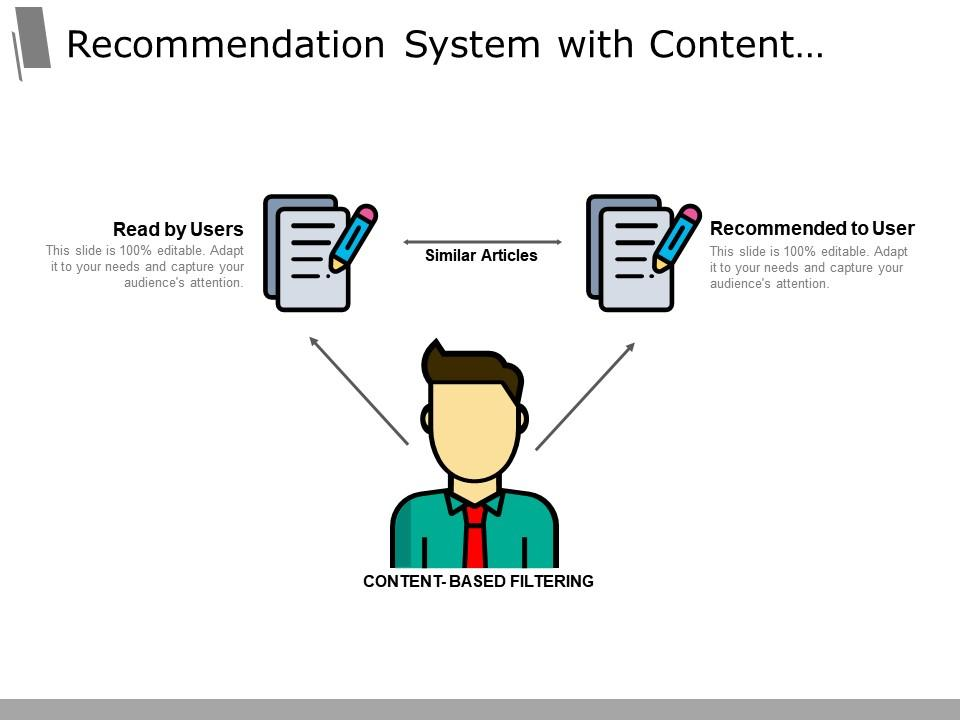
\includegraphics[width=0.65\textwidth]{pic/2}
        \caption{Принцип работы content based фильтрации[6]}
        \label{fig:img1}
    \end{figure}
    \item Коллаборативная фильтрация. Данные модели основаны на идеи поиска похожих пользователей (User based) или объектов (Item based)
    на основе истории взаимодействий. Главными минусами такого подхода является большее время на обучения модели и отсутствие учета содержимого объектов рекомендации.
    \begin{figure}[H]
        \centering
        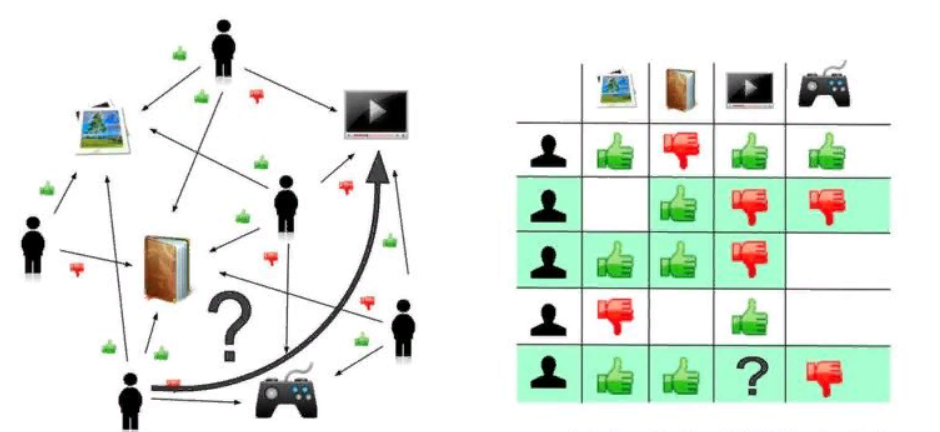
\includegraphics[width=0.7\textwidth]{pic/1}
        \caption{Принцип работы коллаборативной фильтрации[5]}
        \label{fig:img1}
    \end{figure}
    \item Гибридная фильтрация. Как понятно из названия, данные методы совмещают в себе предыдущие, сохраняя их сильные
    стороны, представляя из себя ансамбли из предыдущих моделей. Единственный минус таких моделей это необходимость 
    больше времени на обучения, что нивелируется более высокими метриками.
    \begin{figure}[H]
        \centering
        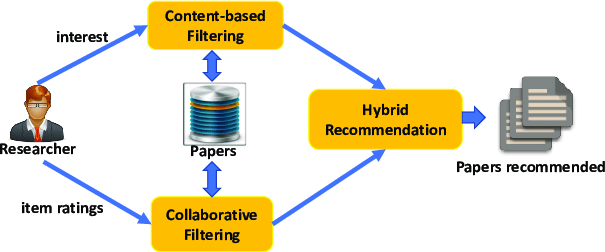
\includegraphics[width=0.7\textwidth]{pic/3}
        \caption{Принцип работы гибридной фильтрации[3]}
        \label{fig:img1}
    \end{figure}
\end{enumerate}

В данный промежуток времени первые два подхода являются хорошо изученными и модели, относящиеся к ним называются
моделями первого уровня. Эксперименты с гибридными архитектурами же продолжаются. Другими словами основное развитие
в сфера рекомендательных систем сегодня заключается в поисках такой архитектуры, которая сможет лучше всего использовать
результаты моделей первого уровня.

Стоит отметить, что выбор модели для ранжирования зависит не только от качества модели, но и от позиционирования
этой модели в сервисе. Т.е., например, если для сервиса необходима рекомендация объекта похожего на тот, с которым пользователь
взаимодействует в данный момент лучше всего подойдут модели, основанные на содержимом объекта.
\subsubsection{Рекомендация популярного}
Данная модель является хорошим бейзлайном для данного класса задач, а также хорошей моделью для построения
рекомендаций для холодных пользователей, так как не требует информации об истории взаимодействий пользователя.
Но это же и является главным минусом такого подхода: такие рекомендации будут являться неперсонализированными,
т.е. всем пользователям будут рекомендоваться одни и те же объекты, что чревато плохим качеством рекомендаций.

Данный подход можно улучшить за счет добавления простых правил. Например, рекомендации объектов популярных у
возрастной группы, к которой относится пользователь и т.д. Такой подход требует больше информации о пользователе,
но при этом качество рекомендаций будет гораздо выше. Однако, такая модель также является неперсонализированной,
при этом требует более тщательного анализа данных и проигрывает по качеству моделям, в основе которых лежит машинное
обучение.

Такой способ рекомендаций сложно отнести к какой либо из вышеописанных категории моделей, но результаты полученные
с помощью него часто также применяют для переранжирования рекомендаций.
\subsubsection{Content based модели}
Модели данного типа сильно зависят от самого контента, на рекомендацию которого нацелена система. В большинстве случаев
основная сложность построение таких систем ранжирования, заключается в поиске способов представления объектов в математическом
пространстве, чтобы вместе со степенью отличия росло и расстояние между объектами в этом пространстве. Иными словами
основная задача заключается в построение грамотных эмбеддингов объектов, а нахождение похожих объектов по ним уже не
составляет большой проблемы. Для этого подойдет простейший алгоритм поиска ближайших соседей.

\begin{figure}[H]
    \centering
    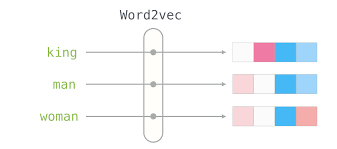
\includegraphics[width=0.7\textwidth]{pic/5}
    \caption{Пример получение эмбеддинга слов с помощью Word2Vec[7]}
    \label{fig:img1}
\end{figure}

Получения хороших эмбеддингов текстов является первым этапом задач NLP (Natural Language Processing), поэтому данный тип
контента представлять в виде вектора проще всего. Для этого используются такие энкодеры как BERT, Word2Vec, TFIDF, FastText и другие.

Техника представления изображений является более сложной. Для получения их эмбеддинга обычно обучают некоторую модель сверточной нейронной сети для
классификации, чтобы взять результат с одного из ее последних слоев. Однако, совсем недавно миру были продемонстрированы такие модели
для работы с изображениями как VIT и DeIT. В основе их архитектуру лежит архитектура transformer, созданная изначально для NLP задач.
Сама архитектура моделей в данной работе не представляет такой интерес, как энкодинг изображения для подачи в нее. Изначально,
перед подачи изображения в сети ее представляют в виде вектора аналогично тексту. Для этого ее разбивают на несколько
частей, где преобразование каждой части эквивалентно преобразованию слова в NLP энкодере.

Метод работы с видеоданными в content based системах аналогичен работе с изображениями, так как видео представляет
из себя просто набор фрэймов (изображений). Поэтому видеоданные представляется либо вектором эмбеддингов всех его фреймов,
либо их суммой, либо их усреднением.

Хорошее представление же аудио данных является нерешенной задачей и по сей день. Существуют такие экспериментальные
методы как преобразование Фурье и спектрограммы. Однако большое количество работ в этой области показало не очень
хорошие результаты.
\subsubsection{Коллаборативная фильтрация}
В основе таких моделей лежит SVD разложение матрицы взаимодействий($M$) пользователей с объектами на две матрицы ($U$ и $V$),
произведение которых вернет исходную матрицу взаимодействия. Однако вследствие того, что в матрице взаимодействий присутствует много
пропусков (т.к. не существует даже одного пользователя, которые полностью провзаимодействовал со всеми объектами
и наоборот), классические алгоритмы SVD разложения не используются, чтобы не потерять информацию о пока что отсутствующих
взаимодействиях. Для этой задачи используют поиск приближенного SVD разложения, который заключается в минимизации
функции 
\begin{equation}
    M_{n\times m} = UVmin(\sum_{i,j}(m_{i,j}-u_i \times v_j)),
\end{equation}
где $u_i$, $v_j$ строки и столбцы матриц $U$ и $V$ соответственно, $m_{i,j}$ - известные элементы матрицы $M$.
Минимизация может производиться различными математическими методами, например, с помощью градиентного спуска.

По факту полученные матрицы представляет из себя эмбеддинги пользователей и объектов, а вследствие того, что это приближение,
то на практике при их произведении получится приближенная матрица взаимодействия, т. е.

\begin{equation}
    U \times V \approx M.
\end{equation}

В следствие этого факта на местах пропусков появятся значения и при выдаче рекомендации нужно просто
выдать объекты, которые будут иметь максимальное значение в аппроксимированной матрице взаимодействия
и с которыми еще не взаимодействовал пользователь. Данный способ использования эмбеддингов является
гибридным, так как учитывает и схожесть пользователей и схожесть объектов, но является самым долгим,
так как операция умножения матриц имеет кубическую сложность.

По полученным эмбеддингам можно также производить поиск похожих пользователей или объектов (например с
помощью алгоритма ближайших соседей). Данные способы являются менее эффективными, но занимают меньше
времени для расчета рекомендаций нескольких пользователей ($O(km)$, где $k$ - это размер эмбеддинга,
а $m$ - количество объектов). Однако при расчете рекомендаций для всх пользователей будет получено
такое же время работы, как и при умножении матриц. Но даже в этом случае можно ускорить этот расчет
используя аппроксимацию ближайших соседей с помощью одной из следующих структур данных:

\begin{enumerate}
    \item Граф.
    \item Дерево.
    \item Хэш корзины.
\end{enumerate}

Главным минусом коллаборативной фильтрации является невозможность ее применения для получения эмбеддингов холодных
пользователей и объектов. Но существуют некоторые алгоритмы, которые по признакам пользователя или объекта,
могут выдавать хороший эмбеддинг. Так, например, сервис spotify по спектрограмме музыки с помощью нейронных сетей
генерирует ее эмбеддинг, за счет чего происходит продвижение композиций малоизвестных исполнителей.

\subsubsection{Гибридные модели}
Обычно такие модели представляют из себя ансамбль, где на первом уровне находятся вышеописанные модели,
генерирующие параллельно списки рекомендованных объектов для пользователей и признаки в виде эмбеддингов
пользователь, объектов и содержимого объектов, а на втором некоторая модель занимается переранжированием объектов в этом списке.
Такая модель чаще всего представляет из себя классификатор, который выдает вероятность того, что пользователь провзаимодействует
с объектом. Такая архитектура позволяет не только получить дополнительные признаки, но и сократить время
на обучения и выдачу прогноза классификатора. При этом подход с классификатором является неединственным.
На смену ему приходят более сложные механизмы, которые показывают результаты лучше. Например, социальные
сети на основе результатов моделей первого уровня строят граф и используют проход по нему с помощью
алгоритмов случайных блужданий.

\begin{figure}[H]
    \centering
    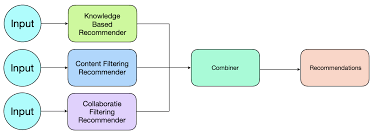
\includegraphics[width=0.6\textwidth]{pic/4}
    \caption{Двухуровневая архитектура[4]}
    \label{fig:img1}
\end{figure}


В данной работе будут рассмотрена только классическая архитектура с классификатором в виде механизма
переранжирования. Такая архитектура учится следующим образом: сначала происходит обучение моделей первого уровня,
затем находится пример положительного взаимодействия пользователя
с объектом и для этого примера этими моделями генерируется еще несколько примеров отрицательного
взаимодействия. Таким образом генерируется большая конечная выборка, после чего на ней происходит обучение
модели второго уровня.

В качестве переранжирующей модели можно использовать любой классификатор, но лучше себя показывают архитектуры
градиентного бустинга и нейронные сети, так как первые хорошо и быстро работают с большим количеством признаков,
а вторые можно очень гибко настроить с помощью кропотливого подбора слоев.

\subsection{Оценка качества рекомендательной системы}

Как и в других сферах машинного обучения, оценка качества рекомендаций проходит в два этапа:

\begin{enumerate}
    \item Оценка в офлайне на данных, которые уже существуют. На данном этапе принимается решение о
    целесообразности применения нового подхода в реальных условиях. За счет этого сразу отсекаются
    модели, которые выдают плохие метрики.
    \item Оценка в онлайне с помощью A/B тестирования. На данном этапе уже идет сравнение с используемой
    в данной момент моделью, чтобы понять на сколько лучше/хуже работает новая модель.
\end{enumerate}

Стоит отметить, что не всегда высокие метрики в онлайне хорошо коррелируют с высокими метриками в офлайне.
При этом модели рекомендательных систем больше всего подвержены ухудшению качества со временем, чем их собратья
из других сфер, из-за чего их нужно переобучать раз в какой-то период, что тоже влияет на принятие решения
об их имплементации в качестве новых основных моделей.

Существует множество метрик, по которым сравнивается качество работы моделей. Основными из них являются 
MAP@k(Mean Average Precision at k) и nDCG@k(normalized Discounted Cumulative Gain at k). Они обе принимают значения в диапозоне [0,1],
где чем больше значение, тем лучше работа модели, и показывают
насколько хорошо ранжирование результатов соответствует предпочтениям пользователя, а разница между ними заключается
в том, что первую метрику используют в случае бинарных значений эталонной релевантности, а вторую в случае
небинарных.

Существуют также более продвинутые метрики, которые учитывают уникальность и полноту охвата рекомендаций.

\subsubsection{Mean Average Precision at k}
Пусть архитектура выдает k элементов в качестве рекомендации. В этом случае самой простой метрикой, которую
можно рассчитать для одного примера будет precision at k (p@k):

\begin{equation}
    p@k = \frac{\text{количество релевантных элементов}}{k}.
\end{equation}

Проблема данной метрики заключается в том, что она не учитывает позиции элементов в топе. Так две модели, которые
выдают одну релевантную рекомендацию будут иметь одинаковые метрики, даже, если первая модель выдает релевантную
рекомендацию на первом месте топа, а вторая на последнем. Очевидно, что в данном случае вторая модель проигрывает
первой по качеству.

Для того, чтобы подобной проблемы не возникало была создана метрика average precision at k (ap@k):

\begin{equation}
    ap@k = \frac{1}{k}\sum_{i=1}^{k}r_ip@i,
\end{equation}

где $r_i$ принимает значение 1, в случае если $i$ элемент топа является релевантным, и 0 в обратном случае.

Выше описанные метрики применяются для оценки качества рекомендаций для одного пользователя. Для того, чтобы
вычислить качество ранжирования для $n$ пользователей берут среднее от суммы оценок ap@k для них. Данная метрика
и называется mean average precision at k и имеет формулу:

\begin{equation}
    map@k = \frac{1}{n}\sum_{i=1}^{n}ap@k_j.
\end{equation}

\subsubsection{Normalized Discounted Cumulative Gain}
В случае, если эталонные значения являются небинарными (например, оценки объектов), то лучше использовать
данную метрику. Она вычисляется по следующей формуле

\begin{equation}
    nDCG@k = \frac{DCG@k}{IDCG@k},
\end{equation}
где DSG@k вычисляется путем суммирования релевантностей всех результатов, учитывая их порядок в списке путем домножения релевантности элемента на вес равный обратному логарифму номера позиции, т.е.

\begin{equation}
    DCG@k = \sum_{i=1}^p\frac{2^{r_i} - 1}{log_2(i+1)},
\end{equation}
а IDCG@k вычисляется аналогично, но с учетом идеального порядка результатов.
\section{Практическая часть}
\conclusion 
/
\begin{thebibliography}{99}
    \bibitem{1}
    Пять технологий искусственного интеллекта, о которых вам нужно знать [Электронный ресурс] – URL: https://www.sas.com/ru_ru/insights/articles/analytics/five-ai-technologies.html (дата обращения 27.04.2021) - Загл. с экрана. Яз. рус.
    \bibitem{2}
    Нейронные сети для начинающих. Часть 1 [Электронный ресурс] – URL: https://habr.com/ru/post/312450/ (дата обращения 13.05.2022) - Загл. с экрана. Яз. рус.
    \bibitem{3}
    A Guide to Building Hybrid Recommendation Systems for Beginners [Электронный ресурс] – URL: https://analyticsindiamag.com/a-guide-to-building-hybrid-recommendation-systems-for-beginners/ (дата обращения 01.05.2022) - Загл. с экрана. Яз. англ.
    \bibitem{4}
    Building a hybrid recommendation system for Jokes recommendations [Электронный ресурс] – URL: https://www.oreilly.com/library/view/advanced-machine-learning/9781838641771/0aa25981-d582-4347-9928-2d967133822e.xhtml (дата обращения 01.05.2022) - Загл. с экрана. Яз. англ.
    \bibitem{5}
    Коллаборативная фильтрация простыми словами [Электронный ресурс] – URL: https://lala.lanbook.com/kollaborativnaya-filtraciya-prostymi-slovami (дата обращения 01.05.2022) - Загл. с экрана. Яз. рус.
    \bibitem{6}
    Recommendation system with content based filtering [Электронный ресурс] – URL: https://www.slideteam.net/recommendation-system-with-content-based-filtering.html (дата обращения 01.05.2022) - Загл. с экрана. Яз. англ.
    \bibitem{7}
    Word2vec в картинках [Электронный ресурс] – URL: https://habr.com/ru/articles/446530/ (дата обращения 01.05.2022) - Загл. с экрана. Яз. рус.
    \bibitem{8}
    Рекомендательные системы: продвинутые алгоритмы [Электронный ресурс] – URL: https://www.bigdataschool.ru/blog/recommender-systems-advanced-algorithms.html (дата обращения 01.05.2022) - Загл. с экрана. Яз. рус.
    \bibitem{9}
    Рекомендательные системы: что это и как работает алгоритм рекомендаций [Электронный ресурс] – URL: https://mindbox.ru/academy/education/rekomendatelnye-sistemy/ (дата обращения 01.05.2022) - Загл. с экрана. Яз. рус.
    \bibitem{10}
    Метод ближайших соседей [Электронный ресурс] – URL: http://www.machinelearning.ru/wiki/index.php?title=Метод_ближайшего_соседа (дата обращения 01.05.2022) - Загл. с экрана. Яз. рус.
    \bibitem{11}
    A/B тест — это просто [Электронный ресурс] – URL: https://habr.com/ru/articles/233911/ (дата обращения 01.05.2022) - Загл. с экрана. Яз. рус.
    \bibitem{12}
    Градиентый бустинг — просто о сложном [Электронный ресурс] – URL: https://neurohive.io/ru/osnovy-data-science/gradientyj-busting/ (дата обращения 01.05.2022) - Загл. с экрана. Яз. рус.
    \bibitem{13}
    Ансамбли в машинном обучении [Электронный ресурс] – URL: https://academy.yandex.ru/handbook/ml/article/ansambli-v-mashinnom-obuchenii (дата обращения 01.05.2022) - Загл. с экрана. Яз. рус.
    \bibitem{14}
    Метрики качества ранжирования [Электронный ресурс] – URL: https://habr.com/ru/companies/econtenta/articles/303458/ (дата обращения 01.05.2022) - Загл. с экрана. Яз. рус.
    \bibitem{15}
    Normalized Discounted Cumulative Gain [Электронный ресурс] – URL: https://towardsdatascience.com/normalized-discounted-cumulative-gain-37e6f75090e9 (дата обращения 01.05.2022) - Загл. с экрана. Яз. англ.
\end{thebibliography}

\appendix

    %\section{Код environment.py}
    %\inputminted[fontsize=\footnotesize]{text}{../environment.py}

    %\section{Код train.py}
    %\inputminted[fontsize=\footnotesize]{text}{../trainer.py}

    %\section{Код test.py}
    %\inputminted[fontsize=\footnotesize]{text}{../test.py}

\end{document}